%% 4. 「技術研究報告」
\documentclass[technicalreport]{ieicej}

\bibliographystyle{ieeetr}
%\usepackage{graphicx}
%\usepackage{latexsym}
\usepackage[dvipdfmx]{color}
\usepackage[dvipdfmx]{graphicx}
\usepackage{amsmath,amssymb,amsfonts}
%\usepackage{cite}
%\usepackage[psamsfonts]{amssymb}

\jtitle{フェージング環境におけるプライマリユーザ信号の時間的変化\\を考慮したデータベース精度向上法の検討}
\jsubtitle{}
\etitle{Accuracy Improvement for Spectrum Database considering\\Primary Signal in Time Domain Under Fading Environment}
\esubtitle{}
\authorlist{%
 \authorentry[wang\noexpand\noexpand\noexpand\_h@awcc.uec.ac.jp]{王\,\,\,\,\,\,昊}{Hao WANG}{awcc}% <= 記述しないとエラーになります
 \authorentry[k\noexpand\noexpand\noexpand\_sato@awcc.uec.ac.jp]{佐藤 光哉}{Koya SATO}{awcc}
 \authorentry[fujii@awcc.uec.ac.jp]{藤井 威生}{Takeo FUJII}{awcc}
}
\affiliate[awcc]{電気通信大学 先端ワイヤレス・コミュニケーション研究センター\\〒182-8585 東京都調布市調布ケ丘1丁目5-1}{Advanced Wireless and Communication research Center, The University of Electro-Communications,\\ 1-5-1 Chofugaoka, Chofu, Tokyo 182-8585, Japan}
%\affiliate[所属ラベル]{和文勤務先\\ 連絡先住所}{英文勤務先\\ 英文連絡先住所}
%\affiliate[所属ラベル]{和文勤務先\\ 連絡先住所}{英文勤務先\\ 英文連絡先住所}

\begin{document}
\begin{jabstract}
%和文あらまし
 コグニティブ無線を用いた周波数共用において,実用的な電波環境推定技術として電波環境データベースに注目を集めている.これまで車載無線機やスマートフォンといった移動端末が観測した膨大な電波環境情報から各位置における周波数の利用状況を高精度に構築される電波環境データベースが提案されている.
しかし,無線LANのように観測期間内に状態遷移する可能性のあるシステムについては,最終的な平均結果とON状態のみを抽出した平均受信電力値に差が生じる恐れがあった.
そこで本研究では,観測期間内にPUの通信状態が遷移する場合の電波環境データベースの構築について検討を行う.1回の観測期間内での受信電力に関する分布変化を検出することにより,PUの通信状態の遷移点を検出するアルゴリズムを提案する.検出した遷移点を用いて、通信を行なっている状態のみの受信電力値の取り出しが可能となり,PUが通信を行なっている状態での平均受信信号電力値を精度良く推定できる.本稿では特に,有効期間の検出に焦点を当てたシミュレーション評価を行ない,その有効性を示す.
\end{jabstract}
\begin{jkeyword}
%和文キーワード
コグニティブ無線,電波環境データベース,スペクトラムセンシング,遷移点検出
\end{jkeyword}
\begin{eabstract}
%英文アブストラクト
Recently, with the fast development of wireless communication technology, cognitive radio (CR) has been recognized as a promising solution to address the problem of impending spectrum scarity for improving the utilization of spectrum for various wireless applications. In a CR system, it allows the Secondary Users (SUs) to opportunistically utilize the temporal and/or spatial unused spectrum holes without harmful interference to Primary Users (PUs). While SUs can occupy avaliable spectrum holes as long as the corresponding PU is in active, they must immediately evacuate the band as soon as the corresponding PU appears. One of the main chanllenges is to intelligently determine ongoing PU activity to avoid interferece toward PU. SUs can evacuate the band without affecting PU’s activity and opportunistically access the spectrum to maximize the spectrum usage if the information about PU can be obtained in advance. Hence, more information about PU leads to more effective spectrum usage for SUs, and an external device for provding information of PU is necessary. In conventional database construction method, the activity of primary user is considered to be always ON when the sensor uses the spectrum sensing to calculate the received power at each place. However, a state transition may occur during the sensing period, which leads to a reliability degradation of the RED. In this thesis, an active period detection method of primary signal is proposed. In this method, transition point detection is used to detect a distribution change between ON and OFF state with applying CUSUM (cumulative sum) algorithm, GLR (Generalized Likelihood Ratio) algorithm and Peak Detection, which the cumulative sum of log probability density ratio value is calculated to detect the change between two different distribution.  Then an active period is extracted by using the detected transition point. In this thesis, we focus on the transition point detection performance and received power detction performance. From simulation results, the transition point is well detected and the estimated received power is more accurate than the one using the conventional method.

\end{eabstract}
\begin{ekeyword}
%英文キーワード
Cognitive Radio, Radio Environment Database, Spectrum Sensing, Energy Detection,Transition point Detection
\end{ekeyword}
\maketitle

\section{研究背景}
近年,周波数の枯渇問題を解消するための抜本的な対策として,周波数共用におけるコグニティブ無線技術が活発に研究を行われている.コグニティブ無線を用いた周波数共用において,周波数の二次利用者(SU: Secondary User) は既存の周波数割り当てユーザ(PU: Primary User)への干渉を回避する必要がある.その中で自身の通信品質を確保するためには,正確な電波環境推定技術が重要である.従来研究では,本研究室がこれまで車載無線機やスマートフォンといった移動端末が観測した膨大な電波環境情報から構築される実測値に基づく電波環境データベースを提案してきた.テレビ帯域を対象とした実証実験により,従来の距離減衰モデルに基づく手法と比較してPUの平均受信電力値の空間的な分布を精度良く推定できることを明らかにしている.しかし,これまではPUの通信状態のON/OFF遷移を考慮せずに観測値を一意に平均化していた.そのため,無線LANやセルラ通信のように観測期間内に状態遷移する可能性のあるシステムについては,最終的な平均結果とON状態の平均受信電力値に差が生じる恐れがあった.そこで本研究では,観測期間内にPUの通信状態が時間的に遷移する場合の電波環境データベースの構築における精度について検討を行う.1回の観測期間内での受信電力に関する分布変化を検出することにより,PU の通信状態の遷移点を検出するアルゴリズムを提案する.その分布の変化検出にCUSUMアルゴリズムとGLRアルゴリズムが用いられ,2つの分布の累積対数尤度比の変化傾向から遷移点の検出が可能となる.検出した遷移点を用いて,通信を行なっている状態のみの有効期間から受信電力値の取り出しが可能となり,PU が通信を行なっている状態での平均受信信号電力値を精度良く推定できる.本研究では特に,状態遷移の検出性能及び受信電力値の推定性能に焦点を当てたシミュレーション評価を行ない,その有効性を示す.シミュレーションにより,提案手法を用いることで遷移点が精度よく検出され,受信電力値の推定誤差が状態遷移が考慮されていない従来手法より抑えることが可能である.
\begin{figure}[t]
  \centering
  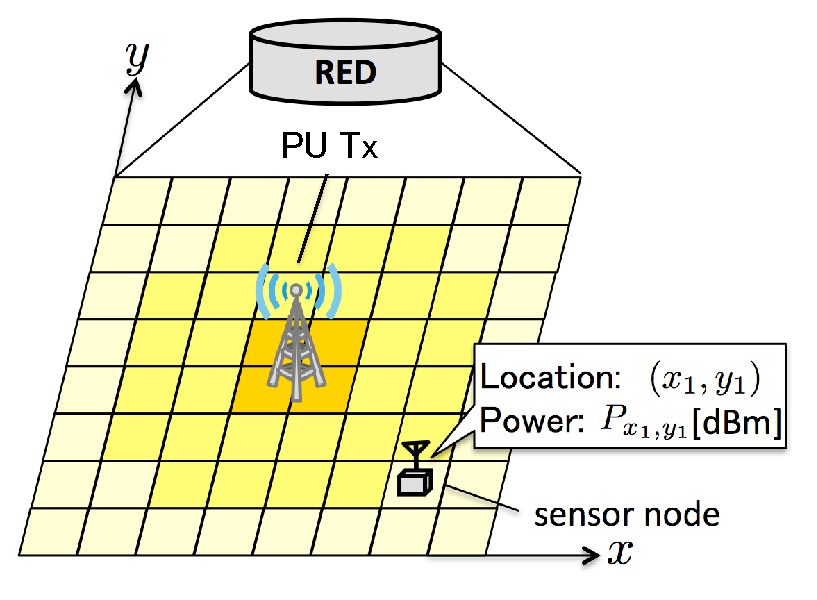
\includegraphics[width=0.8\hsize,clip]{database.eps}
  \caption{電波環境データベース}
  \label{databse}
\end{figure}



\section{システムモデル}
\label{sec:model}
図1に本研究で想定するシステムモデルの概要を示す.本研究では,ONとOFFの2状態遷移するPUが1台ある環境において観測センサ1台が観測を行うこととする.観測センサは観測期間内に$T$サンプルを取得する.PUの時間的通信状態が遷移するため,観測センサが取得したサンプル$y[i]$は式(\ref{sample})のようになる.
\begin{align}
s[i]=
\left\{
\begin{array}{ll}
w[i], & i=1,\dots,\tau_1-1 \\
x[i]+w[i],& i=\tau_1,\dots,\tau_2-1 \\
w[i],& i=\tau_2,\dots,T 
\end{array}
\right.
\label{sample}
\end{align}


\begin{align}
y[i]=
\left\{
\begin{array}{ll}
w[i]*w[i]^{*}\, & i=1,\dots,\tau_1-1 \\
(x[i]+w[i])(x[i]+w[i])^{*},& i=\tau_1,\dots,\tau_2-1 \\
w[i]*w[i]^{*},& i=\tau_2,\dots,T 
\end{array}
\right.
\label{sample}
\end{align}

$\tau_1$と$\tau_2$はそれぞれOFFからONの遷移点(立ち上がり点)とONからOFFの遷移点(立ち下がり点)である.また,$x[i]$はPUの送信信号で,$w[i]$は平均0,分散$\sigma^{2}_{n}$の加法性白色ガウス雑音(AWGN:Additive White Guassian Noise)である.次に,$P$は観測センサにおける受信電力値とする時,PUがOFFとONの時のサンプル値はそれぞれ平均0,分散$\sigma^2$と$\sigma^2+P$の正規分布に従うことを仮定し,確率密度関数(PDF: Probability Density Function)は式(\ref{normal})である.

\begin{align}
\begin{cases}
\;f_0(t) = \frac{1}{\sqrt{2\pi\sigma^2_n}}t^{-\frac{1}{2}} \rm{exp}\left\{{-\frac{t}{2}}\right\} \\
\;f_1(t) = \frac{1}{\sqrt{2\pi\sigma^2_n}} \rm{exp}^{-\frac{(t-P)^2}{2\sigma^2_n}}
\end{cases}
\label{normal}
\end{align}

\begin{figure}[t]
\centering
\includegraphics[width=0.8\hsize,clip]{systemmodel.eps}
\caption{\normalsize{システムモデル}}
\label{systemmodel}
\end{figure}


\section{遷移点検出法}
\label{sec:transition}


\begin{figure}[t]
\centering
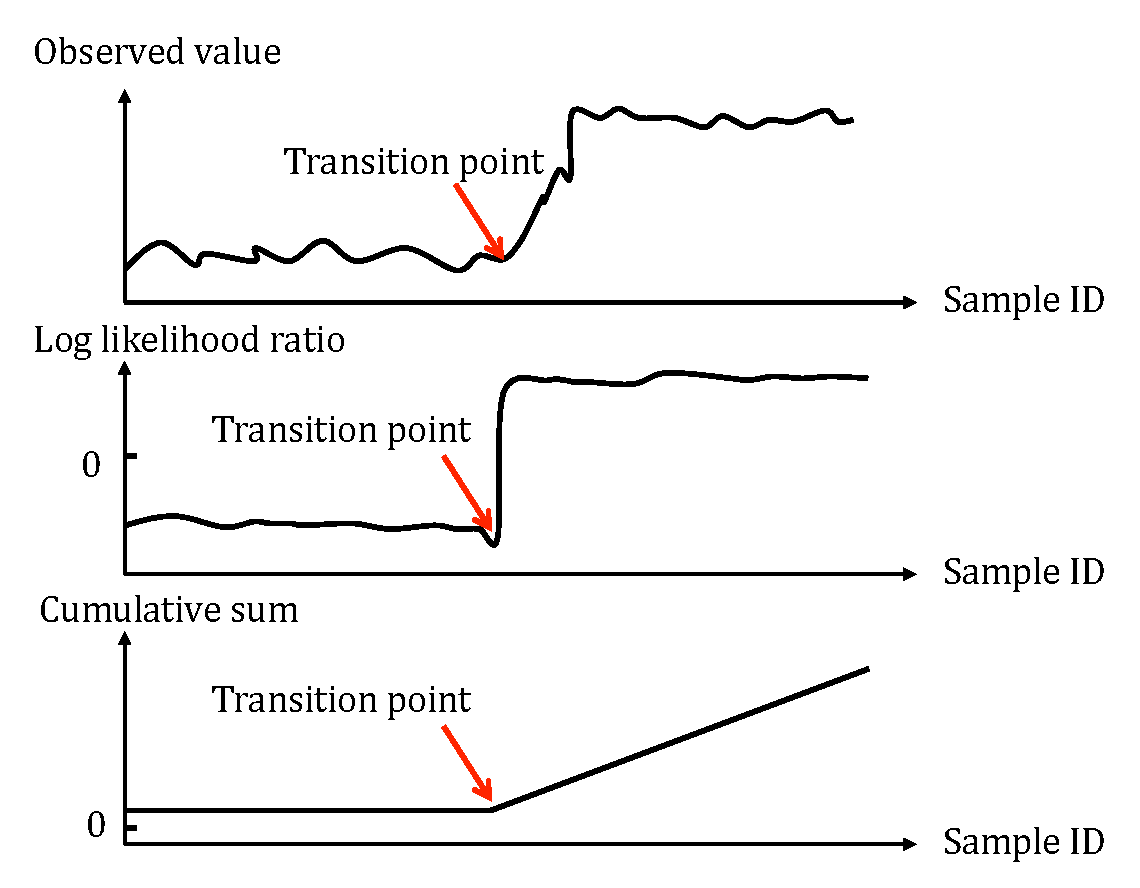
\includegraphics[width=0.8\hsize,clip]{cusum_image.eps}
\caption{遷移点検出のイメージ図}
\label{systemmodel}
\end{figure}
取得した遷移点込みの全サンプルを一意に平均化を行う場合,真の電力値と差分が生じる問題がある.これに対し,OFFからONまたはONからOFFに一回しか遷移しない場合の遷移点検出法が検討されていた\cite{ref:quickest}.本研究ではONとOFFの遷移が複数ある環境を想定した遷移点検出法を提案する.
提案手法では雑音の分散$\sigma^2$が既知で,受信電力値$P$がそれぞれ既知と未知の場合のCUSUM(cumulative sum)とGLR(Generalized Likelihood Ratio)アルゴリズムを用いて遷移点を検出する.分布が既知であるため,ONのPDF対OFFのPDFの対数尤度比$l_{1}(y[i])$とOFFのPDF対ONのPDFの対数尤度比$l_{0}(y[i])$を式(\ref{like1})(\ref{like2})で定義する.
\begin{align}
l_{1}(y[i]) &= {\rm ln}\left\{\frac{f_1(y[i])}{f_0(y[i])}\right\} \label{like1} \\
&=\frac{Py^2[i]}{2(P+\sigma^2)\sigma^2} + \frac{1}{2}{\rm ln}\left\{\frac{\sigma^2}{P+\sigma^2}\right\} \nonumber \\
l_{0}(y[i]) &= {\rm ln}\left\{\frac{f_0(y[i])}{f_1(y[i])}\right\} \label{like2} \\
&=\frac{Py^2[i]}{2(P+\sigma^2)\sigma^2} + \frac{1}{2}{\rm ln}\left\{\frac{\sigma^2}{P+\sigma^2}\right\} \nonumber
\end{align}


OFFとONのみのサンプル値の平均対数尤度比をそれぞれ計算すると,以下の式(\ref{D_f0})と(\ref{D_f1})になる.
\begin{align}
E_{f_0}\left\{l_1(y[i])\right\} &=\int f_0(y){\rm ln}\left\{\frac{f_1(y)}{f_0(y)}\right\}dy \nonumber\\
 &=-D(f_0||f_1)\leq 0 \label{D_f0} \\
E_{f_1}\left\{l_1(y[i])\right\} &=\int f_1(y){\rm ln}\left\{\frac{f_1(y)}{f_0(y)}\right\}dy \nonumber\\
 &=D(f_1||f_0)\geq 0 \label{D_f1}
\end{align}
ここで,$D(f_0||f_1)$と$D(f_1||f_0)$は$f_0$の$f_1$と$f_1$の$f_0$に対するカルバック・ライブラー情報量である.式(4)と(5)をみると,OFFの時のサンプルの対数尤度比は負であり,ONの場合は正である.同様に計算すると,OFFのPDF対ONのPDFの対数尤度比$l_{0}(y[i])$はONの時のサンプルの対数尤度比は負であり,OFFの場合は正である.

\subsection{CUSUMアルゴリズム($\sigma^2$既知,$P$既知)}
式(\ref{D_f0})(\ref{D_f1})の性質を利用すると,対数尤度比の累積和が最大となるように式(\ref{Cusum})を遷移点の判定式として定義する.

\begin{eqnarray}
g_t =  \max_{k \leq t}\left\{\sum_{i=1}^tl(y[i]-\sum_{i=1}^kl(y[i]))\right\}= \max_{k \leq t}\sum_{i=k+1}^tl(y[i])
\label{Cusum}
\end{eqnarray}

$g_t$がある閾値$h$より大きい場合,分布の変化いわばPUの状態遷移発生として検出する.また$P$は既知であるため,$g_t$を式(\ref{rec})のように再帰的に計算可能である.
\begin{eqnarray}
g_{t+1}=\left\{g_t+l(y[t+1]),0\right\}^{+}
\label{rec}
\end{eqnarray}

\subsection{GLRアルゴリズム($\sigma^2$既知,$P$未知)}
$P$が常に既知とは限らないため,ここでは$P$は$[P_{{\rm min}},P_{{\rm max}}]$にあると仮定し,$g_t$の計算は式(\ref{Glr})に従う.

\begin{eqnarray}
g_t &= \max_{k \leq t}\sum_{i=k+1}^tl(y[i])={\rm ln}\left\{\prod_{i=k+1}^k\frac{f_{1,P}(y[i])}{f_0(y[i])}\right\} \\ 
    &= \max_{k \leq t}\sum_{i=k+1}^t\left\{ \frac{Py^2[i]}{2(P+\sigma^2)\sigma^2}+\frac{1}{2} {\rm ln}\left\{ \frac{\sigma^2}{P+\sigma^2}\right\} \right\} 
\label{Glr}
\end{eqnarray}

また,再帰的に計算するのは不可能であるため,以下の式(\ref{fp})として$f(P)$を定義する.
\begin{eqnarray}
f(P) = \frac{P}{2(P+\sigma^2)\sigma^2}\hat{y}+(t-k)\frac{1}{2}{\rm ln}\left\{ \frac{\sigma^2}{P+\sigma^2} \right\} 
\label{fp}
\end{eqnarray}
ここで,$\hat{y}=\sum_{i=k+1}^t y^2[i]$である.次に,範囲$[P_{{\rm min}},P_{{\rm max}}]$内に$f(P)$が最大となる$P$を以下の式(\ref{maxP})によって決定する.

\begin{equation}
P^{*}=
\left\{
\begin{array}{ll}
P_{{\rm max}}, & (t-k)\leq\frac{\hat{y}}{P_{{\rm max}}+\sigma^2}, \\
\frac{\hat{y}}{t-k}-\sigma^2, & \frac{\hat{y}}{P_{{\rm max}}+\sigma^2}\leq(t-k)\leq\frac{\hat{y}}{P_{{\rm min}}+\sigma^2}, \\
P_{{\rm min}}, & (t-k) \geq \frac{\hat{y}}{P_{{\rm min}}+\sigma^2}.
\end{array}
\right.
\label{maxP}
\end{equation}
式(\ref{maxP})によって得られた$P^{*}$より式(\ref{Glr})に従い,$g_t$を計算することが可能である.
\section{フェージング環境における遷移点検出による有効期間検出}
\label{sec:propose}


\begin{figure}[t]
\centering
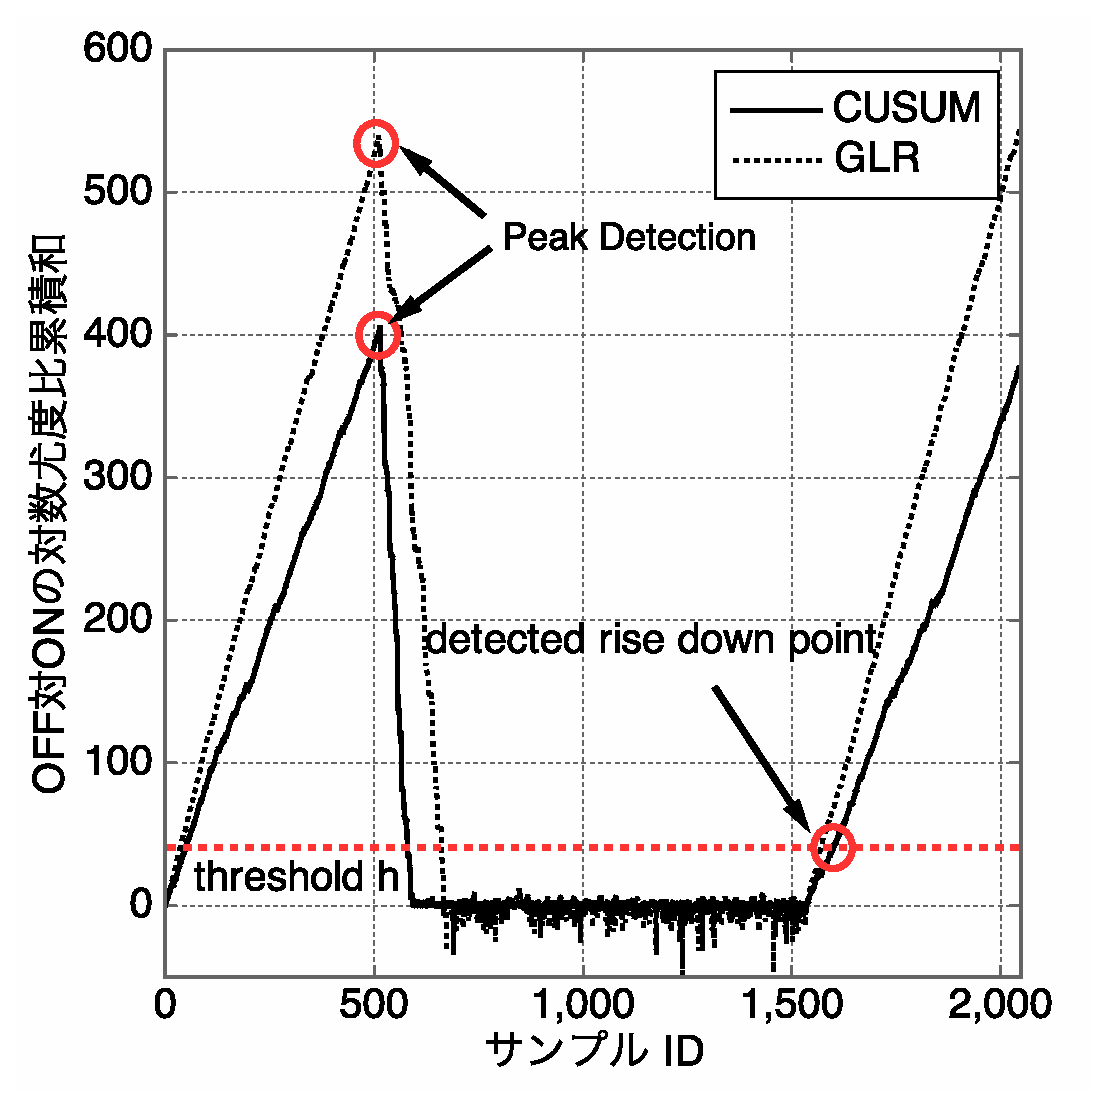
\includegraphics[width=0.8\hsize,clip]{ON2OFF.eps}
\caption{ONのPDF対OFFのPDFの対数尤度比累積和}
\label{sum_up}
\end{figure}

\begin{figure}[t]
\centering
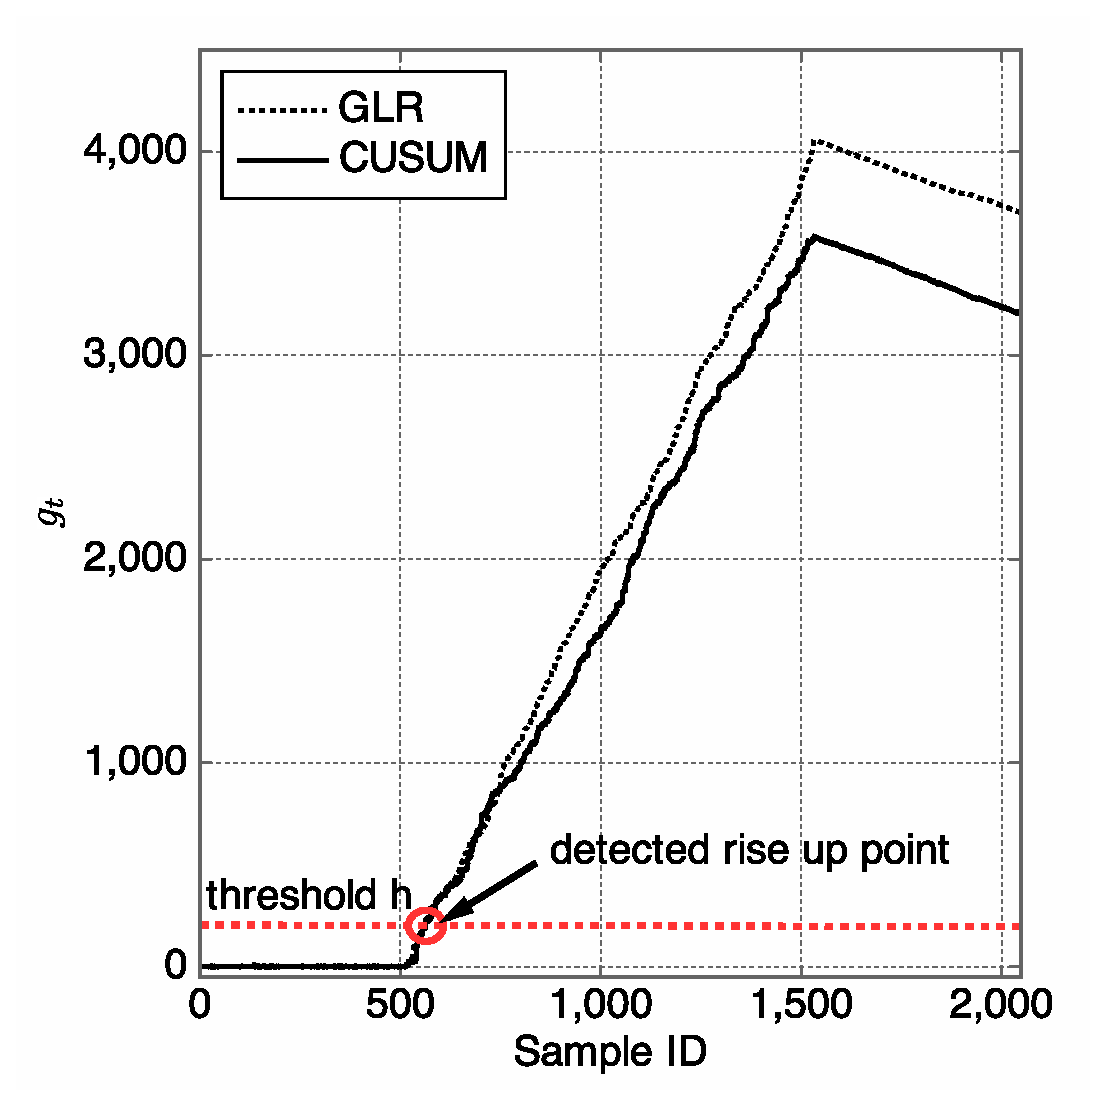
\includegraphics[width=0.8\hsize,clip]{OFF2ON.eps}
\caption{OFFのPDF対ONのPDFの対数尤度比累積和}
\label{sum_down}
\end{figure}


\section{シミュレーション結果及び性能評価}
\label{sec:result}


\begin{figure}[t]
\centering
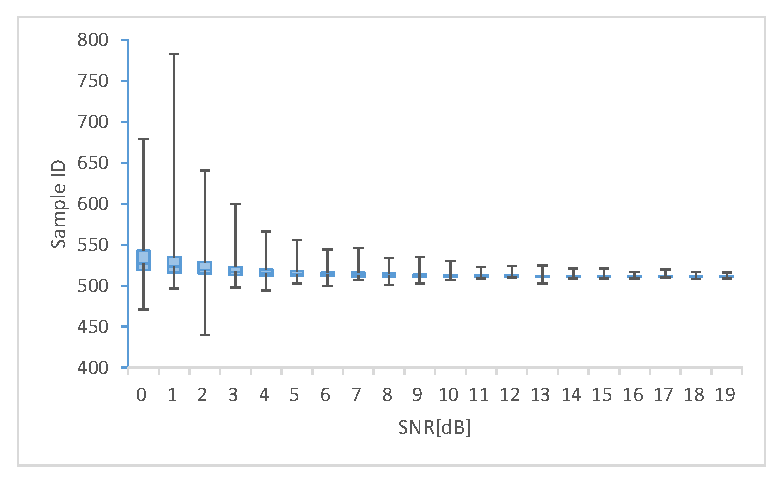
\includegraphics[width=0.8\hsize,clip]{transition_up.eps}
\caption{立ち上がり点の検出性能}
\label{transition_up}
\end{figure}

\begin{figure}[t]
\centering
\includegraphics[width=0.8\hsize,clip]{transition_down.eps}
\caption{立ち下がり点の検出性能}
\label{transition_down}
\end{figure}


\begin{figure}[t]
\centering
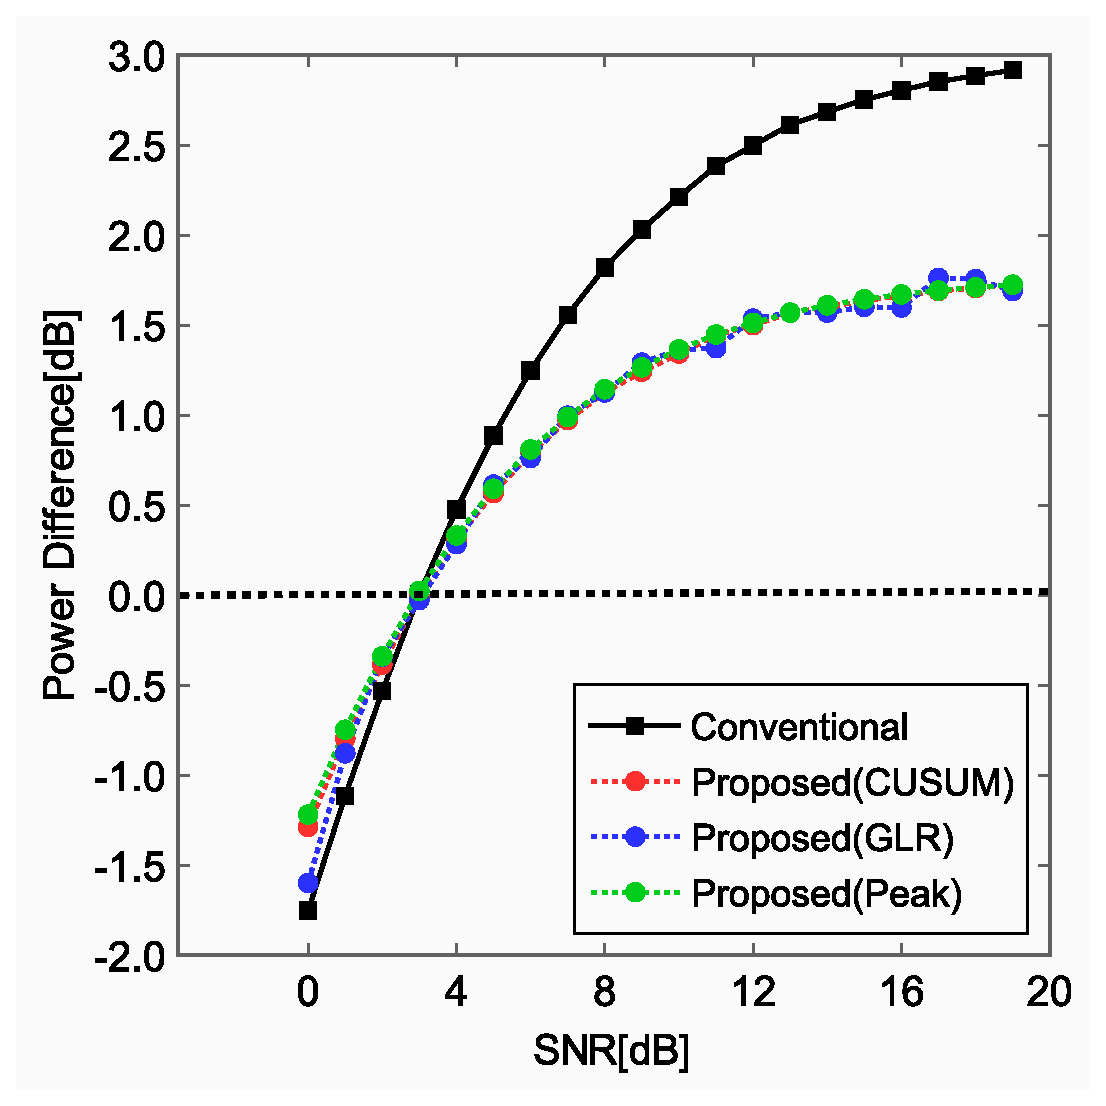
\includegraphics[width=0.8\hsize,clip]{peak.eps}
\caption{提案手法と従来手法の比較.}
\label{peak}
\end{figure}


\section{結論}
\label{sec:conclusion}

\ack

本研究はJSPS科研費15H04004,15H04010の助成を受けたものです.


\bibliographystyle{sieicej}
%\bibliography{myrefs}
 \begin{thebibliography}{10}
\bibitem{ref:Cisco}Cisco, ``Cisco Visual Networking Index: Global Mobile Data Traffic Forecast Update, 2014–2019,''Cisco White Paper.
\bibitem{ref:FCC}Federal Communications Commission, ``Spectrum policy task force report,fcc 02-155,'' Nov. 2002.
\bibitem{ref:mitola}J. Mitola III and G. Q. Maguire, Jr., ``Cognitive radio: making software radios more personal,'' IEEE Personal Communications, vol. 6, no. 4, pp. 13–18, Aug. 1999.
\bibitem{ref:Haykin} S. Haykin, ``Cognitive radio: Brain-empowered wireless communications,'' {\it IEEE J.Selected Areas Commun.},vol. 23, no. 2, pp. 201 - 220, Feb. 2005.
\bibitem{ref:fujii_Database} K. Sato, M. Kitamura, K. Inage, and T. Fujii, ``Measurement-based spectrum database for flexible spectrum management,'' IEICE Trans. Commun., vol.E98-B, no.10, pp.2004-2013, Oct. 2015.
\bibitem{ref:ON1}G. Zhou, J. Wu, K. Sohraby, ``Cooperative Spectrum Sensing with a Progressive MAP Detection Algorithm,'' Proc. GLOBECOM, pp.1-5, Dec. 2011.
\bibitem{ref:ON2}Y. Pei, Y. Liang, K.C.Teh, K. H. Li, ``Sensing-throughput tradeoff for cognitive radio networks: A multiple-channel sceario,'' Proc. IEEE PIMRC, pp.1257-1261, 13-16 Sept. 2009.
\bibitem{ref:quickest}L.Lai, Y.Fan, and H.V.Poor, ``Quickest Detection in Cognitive Radio: A Sequential Change Detection Framework,'' Proc. IEEE Globecom, Dec. 2008.
\bibitem{ref:overlay}Vameghestahbanati, M. and Mir, H.S. and El-Tarhuni, M., `` An overlay architecture for cognitive radio systems,'' Proc. IEEE ICCSPA, pp.1-4, Feb. 2014.
\bibitem{ref:underlay}H. Hu and Q. Zhu, ``Dynamic Spectrum Access in Underlay Cognitive Radio System with SINR Constraints,'' Proc. IEEE WiCompp. 1-4, Sept. 2009.
\bibitem{ref:fcc}Federal Communications Commission, SECOND MEMORANDUM OPINION AND ORDER, Sept. 2010.
\bibitem{ref:google}Google, ``Spectrum database.'' http://www.google.org/spec\\trum/whitespace/, accessed Jan. 15. 2016.
\bibitem{ref:ED}T. Yucek and H. Arslan, ``A survey of spectrum sensing algorithms for cognitive radio applications,'' IEEE {\it Communications Surveys Tutorials}, vol. 11, no. 1, pp. 116-130, 2009.
\bibitem{ref:CUSUM}E. Page, ``Continuous inspection schemes,'' {\it Biometrika}, vol. 41, pp. 100-115, 1954.
\bibitem{ref:GLR}G. Lorden, ``Procedures for reacting to a change in distribution,'' {\it Annals of Mathematical Statistics}, vol. 42, no. 6, pp. 1897-1908, 1971.  
\bibitem{ref:threshold_cusum}G. Lorden, ``ON excess over the boundary,'' {\it Annals of Mathematical Statistics}, vol. 41, pp.520-527, Apr. 1970.
\bibitem{ref:threshold_GLR}G. Lorden, ``Open-ended tests for Koopman-Darmois families,'' {\it Annals of Statistics}, vol. 1, no. 4, pp. 520-527, Apr. 1970.
 \end{thebibliography}
 
\end{document}
